\documentclass[10pt]{beamer}

\usepackage[utf8]{inputenc}
\usepackage[T1]{fontenc}
\usepackage[french]{babel}
\usepackage[ddmmyyyy]{datetime}
\usepackage{listings,lstautogobble,graphicx,tikz,verbatim, amsthm,amsfonts,amsmath,amssymb,mathrsfs,thmtools}
\usetikzlibrary{arrows,automata}
\usetikzlibrary{positioning}

\usetheme{Warsaw}
\useinnertheme{rectangles}
\setbeamerfont{headline}{size=\large}
\setbeamerfont{frametitle}{size=\normalsize}


%Plan/Sommaire automatique avant chaque section
\AtBeginSection[]{
  \begin{frame}
  \frametitle{Plan}
  \tableofcontents[currentsection]
  \end{frame}
}
\AtBeginSubsection[]
{
    \begin{frame}{Plan}
        \tableofcontents[currentsection,currentsubsection]
    \end{frame}
}

\author{Sonny Klotz - Idir Hamad - Younes Benyamna - Malek Zemni}
\institute{UVSQ}
\date{\today}
\usepackage[french,frenchkw,ruled,vlined]{../texLib/algorithm2e}
\usepackage{../texLib/myInfolines}
\usepackage{longtable,array}
\title{Présentation : projet primalité}

\declaretheorem[name=Théorème]{Th}
\declaretheorem[name=Définition]{Def}

\begin{document}

	\begin{frame}
		\titlepage
	\end{frame}
	
	\section*{Introduction}
	
		\begin{frame}
			Projet de M1 informatique UVSQ sur les tests de primalité :\\~\\
			\begin{itemize}
				\item Existence de plusieurs tests de primalité.
				\item Utilisés pour générer des nombres premiers.
				\item Performances différentes.
			\end{itemize}~\\
			\pause
			\textbf{Objectif :} implémentation, description (rapport) et mesures de performances pour construire un générateur optimal.\\
		\end{frame}
	
		\begin{frame}
			\tableofcontents
		\end{frame}
		
	\section{Architecture}
	
		\begin{frame}
		
		Principales fonctionnalités de l'application développée :\\~\\
			\begin{itemize}
				\item Implémentation de tests de primalité :
					\begin{enumerate}
					\item Test Naif
					\item Test de Wilson
					\item Test de Fermat
					\item Test de Miller-Rabin
					\item Test de Solovay-Strassen
					\item Test AKS
					\end{enumerate}
				\item Mesures de performances.
				\item Génération de nombres premiers.
			\end{itemize}~\\
			
		\end{frame}
		\begin{frame}
		Organigramme de l'application et données échangées :\\
			\begin{center}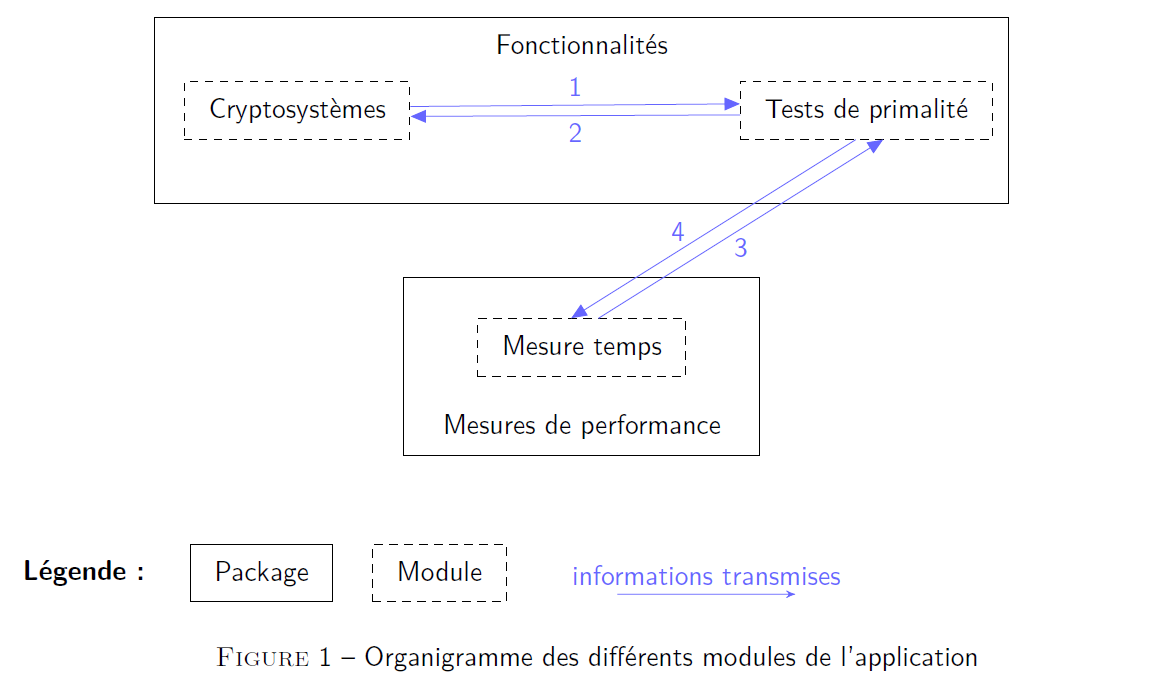
\includegraphics[scale=0.45]{img/org.png}\end{center}
		\end{frame}
		\begin{frame}
		Fonctionnement de l'application :\\~\\
			\begin{itemize}
				\item Mesures de performance de chaque test.
				\item Exploitation des résultats de mesures pour construire le générateur optimal.
				\item Utilisation du générateur par l'utilisateur.
			\end{itemize}
		~\\~\\
		\pause
		Technologies utilisées :\\~\\
			\begin{itemize}
				\item Langage C + GMP
				\item LaTeX
				\item Gnuplot
			\end{itemize}
		\end{frame}
		
	\section{Primalité - cryptosystèmes}
	
		\begin{frame}
			Tests de primalité importants dans la \textbf{cryptographie à clé publique}.\\
			Utilisés pour générer de grands nombres premiers.\\~\\
			\begin{itemize}
			\item \textbf{RSA} : phase de génération des clés.
			\item \textbf{ElGamal} : phase d'échange de clés.
			\end{itemize}
		\end{frame}
		
		\begin{frame}
			Cas de RSA :\\~\\
			\begin{itemize}
			\item Générer 2 grands nombres premiers distincts $p$ et $q$.
			\item Module RSA : $n = p*q$. La taille en bits de $p$ et $q$ est la moitié de celle de $n$.
			\item Calcul de $\phi(n) = (p-1)*(q-1)$.
			\item Clé publique : $e$ premier avec $\phi(n)$.
			\item Clé privée : $d = e^{-1}\pmod\phi(n)$.
			\end{itemize}
			~\\
			Importance des nombres premiers : la \textbf{factorisation} de $n$ permet de retrouver la clé privée $d$.
		\end{frame}
		
	\section{Génération des nombres premiers}
		
		\begin{frame}
			Processus de génération des nombres premiers :\\
			\begin{center}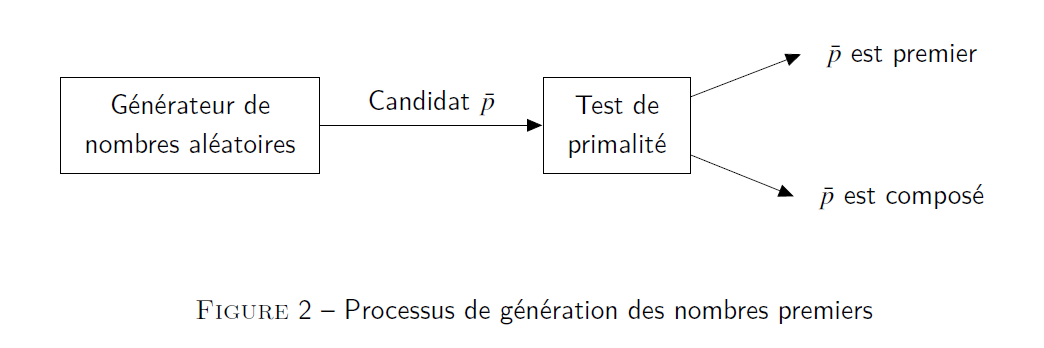
\includegraphics[scale=0.5]{img/gen.png}\end{center}
		\end{frame}
		
		\begin{frame}
			Importance du générateur :\\~\\
			\begin{itemize}
				\item Utilisé par les cryptosystèmes pour générer des nombres premiers.
				\item Importance pour la sécurité : générateur aléatoire imprévisible. 
			\end{itemize}
			~\\
			\pause
			Importance du test de primalité:\\~\\
			\begin{itemize}
				\item Assure que le nombre aléatoire est premier.
				\item Performances du générateur dépend du choix du test de primalité.
			\end{itemize}
		\end{frame}
		
	\section{Tests de primalité}
		\begin{frame}
			Teste si un nombre est \textbf{premier} ou \textbf{composé}.\\~\\
			Existence de plusieurs tests, avec deux type différents :\\
			\begin{itemize}
				\item \textbf{Tests déterministes :} renvoient toujours le bon résultat.
				\item \textbf{Tests probabilistes :} renvoient un résultat avec une certaine probabilité.
			\end{itemize}
			~\\
			\pause
			\begin{table}[H]\begin{center}
				\begin{tabular}{|c|c|c|}
				\hline
				Algorithme           & Année & Type       \\ \hline
				Naïf (Crible d’Eratosthène) & -240  & Déterministe \\ \hline
				Fermat               & 1640  & Probabiliste \\ \hline
				Wilson               & 1770  & Déterministe \\ \hline
				Miller-Rabin         & 1976  & Probabiliste \\ \hline
				Solovay-Strassen     & 1977  & Probabiliste \\ \hline
				AKS                  & 2002  & Déterministe \\ \hline
				\end{tabular}
			\end{center}\end{table}
			
		\end{frame}
		
		\subsection{Test Naïf}
			\begin{frame}
				Méthode la plus intuitive de tester si un nombre est premier ou composé, à laquelle on a effectué plusieurs optimisations :\\~\\
				\begin{center}
				\begin{algorithm}[H]
					\caption{Test naïf}\label{TN}
					\Donnees{un entier $n$}
					\Pour{tout nombre premier $p \leqslant \sqrt{n}$}{
						\Si {$p$ divise $n$}
							{\Retour composé\;}
					}
				\Retour premier\;
				\end{algorithm}
				\end{center}
				~\\
				\textbf{Complexité :} $O(\sqrt{n})$ opérations.
			\end{frame}
		
			\begin{frame}
				Utilisation du \textbf{crible d’Eratosthène} (III\up{e} siècle av. J.-C.) pour pré-calculer et stoker dans une table tous les nombres premiers $\leqslant \sqrt{n}$ :\\~\\
				\begin{center}
					\begin{algorithm}[H]
					\caption{Crible d'Eratosthène}\label{Eras}
					\Donnees{un entier $N$ qui correspond à $\sqrt{n}$}
					{Créer une liste L de couples \textit{(entier, primalité)}, pour les entiers allant de $2$ jusqu'à $N$, avec une primalité initialisée à "premier" : \textit{\textbf{L = \{(2, premier), (3, premier), ..., ($N$, premier)\}}} \;}
					{\textit{\textbf{plusGrandPremier}} = $N$ \;}
					\Pour{tout nombre $p$ marqué "premier" de la liste L (de manière croissante)}{
						\Si{$p^{2}$ > \textit{\textbf{plusGrandPremier}}}{ 
							\Retour L\;
						}
						{\textit{\textbf{i}} = $2$ \;}
						\Tq{$p*i < N$}{ 
							{Marquer "composé" l'entier à la position $p*i$ \;}
							{Mettre à jour \textit{\textbf{plusGrandPremier}} \;}
							{$i++$ \;}
						}
					}
				\end{algorithm}	
				\end{center}
			\end{frame}
			
		\subsection{Test de Wilson}
			\begin{frame}
				Test basé sur une propriété simple : \\~\\
				\begin{center}
				\begin{Th}[Théorème de Wilson]
					Un entier $n > 1$ est un nombre premier si et seulement si
					\[(n-1)! + 1 \equiv 0 \pmod n\]
				\end{Th}
				\end{center}
			\end{frame}
			
			\begin{frame}
				\begin{center}
				\begin{algorithm}[H]
					\caption{Test de Wilson}\label{Wil}
					\Donnees{un entier $n$}
					\Si{$(n-1)! + 1 \equiv 0 \pmod n$} { 
						{\Retour premier\;}
					} \Sinon{
						{\Retour composé\;}
					}
				\end{algorithm}	
				\end{center}
				~\\
				\textbf{Complexité :} $O(n)$.
			\end{frame}
			
		\subsection{Test de Fermat}
			\begin{frame}
				Test de primalité probabiliste basé sur le petit théorème de Fermat :
				\begin{center}
				\begin{Th}[Petit théorème de Fermat (énoncé 1)]
					\label{ThFermat1}
					Si $p$ est un nombre premier, alors pour tout nombre entier $a$ premier avec $p$
					\[a^{p-1}\equiv 1 \pmod p\]
				\end{Th}
				\end{center}
				~\\
				Énoncé la première fois en 1640 par \textit{Pierre de Fermat}.
			\end{frame}
			
			\begin{frame}
				\begin{itemize}
				\item Choix de $1 < a < n$.
				\item Calcul de $\mathbf{a^{n-1} \pmod n}$.
				\item $k$ répétitions.
				\end{itemize}
				\begin{center}
				\begin{algorithm}[H]
					\caption{Test de Fermat}\label{TF}
					\Donnees{un entier $n$ et le nombre de répétitions $k$}
					\Pour{$i$ = $1$ jusqu'à $k$}{
						Choisir aléatoirement $a$ tel que $1 < a < n$\;
						\Si {$a^{n-1} \not\equiv 1 \pmod n$}
							{\Retour composé\;}
					}
				\Retour probablement premier\;
				\end{algorithm}
				\end{center}
			\end{frame}
			
			\begin{frame}
				Présence de nombres \textbf{pseudo-premiers} et nombres de \textbf{Carmichael}.\\~\\
				\begin{Def}[Nombre pseudo-premier]
					\label{PseudoPrem}
					Un nombre pseudo-premier est un nombre premier probable (un entier naturel qui partage une propriété commune à tous les nombres premiers) qui n'est en fait pas premier. Un nombre pseudo-premier provenant du théorème de Fermat est appelé nombre pseudo-premier de Fermat.
				\end{Def}
				~\\
				\begin{Def}[Nombre de Carmichael]
					\label{Carmich}
					Un entier positif composé $n$ est appelé nombre de Carmichael si pour tout entier $a$ premier avec $n$,
					\[a^{n-1}\equiv 1 \pmod n\]
				\end{Def}
			\end{frame}
			
			\begin{frame}
				\textbf{Complexité :} dépend de \\~\\
				\begin{itemize}
				\item l'exponentiation modulaire \textbf{\textit{Square And Multiply}} : ...
				\item la multiplication modulaire : $C_{mult}(n)$
				\end{itemize}
				~\\
				$\Longrightarrow$ Complexité test de Fermat : $O(k \cdot log_{2}(n) \cdot C_{mult}(n))$.
			\end{frame}
		
		\subsection{Test de Miller-Rabin}
			\begin{frame}
		
			\end{frame}
			
			\begin{frame}
		
			\end{frame}
			
			\begin{frame}
		
			\end{frame}
		
		\subsection{Test de Solovay-Strassen}	
			\begin{frame}
		
			\end{frame}
			
			\begin{frame}
		
			\end{frame}
			
			\begin{frame}
		
			\end{frame}	
		
		\subsection{Test AKS}	
			\begin{frame}
		
			\end{frame}
			
			\begin{frame}
		
			\end{frame}
			
			\begin{frame}
		
			\end{frame}	
		
	\section{Mesures de performance et comparatifs}	
		\begin{frame}
	
		\end{frame}
		
		\begin{frame}
	
		\end{frame}
		
		\begin{frame}
	
		\end{frame}
	
\end{document}
